\documentclass{article}   	% use "amsart" instead of "article" for AMSLaTeX format
\usepackage[margin=1in]{geometry}                		% See geometry.pdf to learn the layout options. There are lots.
\geometry{letterpaper}                   		% ... or a4paper or a5paper or ... 
%\geometry{landscape}                		% Activate for for rotated page geometry
%\usepackage[parfill]{parskip}    		% Activate to begin paragraphs with an empty line rather than an indent
\usepackage{graphicx}				% Use pdf, png, jpg, or eps§ with pdflatex; use eps in DVI mode
								% TeX will automatically convert eps --> pdf in pdflatex		
\usepackage{amssymb}
\usepackage{amsmath}
\usepackage{multicol}
\usepackage{enumitem}
\usepackage{color}
\usepackage{hyperref}
\usepackage{tcolorbox}
\usepackage{arydshln}
\usepackage{pifont}
\usepackage{tikz}
\usetikzlibrary{calc,angles,quotes}
\usepackage{siunitx}


\usepackage{fancyhdr}
\pagestyle{fancy}
\rfoot{}
\chead{}
\lfoot{}
\lhead{PHYS 2350 \\ Fall 2024}
\rhead{\thepage}
\cfoot{}

\title{Kenyan Pirates \textrm{I}}
\author{Dr. Wolf}
%\date{}							% Activate to display a given date or no date

\setlength{\parindent}{0pt}

\begin{document}
% \maketitle
% \section{}
% \subsection{}

\begin{tcolorbox}[colback=black!5!white,colframe=white!15!black,title=Problem Context]
  While on a vacation to Kenya, you visit the port city of Mombassa on the Indian Ocean. On the
  coast, you find an old Portuguese fort probably built in the 16\textsuperscript{th}
  century. Large stone walls rise vertically from the shore to protect the fort from cannon
  fire from pirate ships.  You wonder how close a pirate ship would have to sail to the fort to
  be in range of the fort's cannon. Of course you realize that the range depends on the
  velocity that the cannonball leaves the cannon, as well as the height of the cliff.
\end{tcolorbox}

\section{Setting up the problem}
\begin{enumerate}
  \item Below is a schematic drawing of the fort. Choose an origin and coordinate system that
  you will use to describe this motion, as well as any forces that are important for this
  system. To help guide your eye, I have included the initial velocity vector on this schematic
  $\vec{v}_i$, as well as the launch angle $\theta$ which is relative to the horizontal. I've
  also labeled the cliff's height as $H$.
  Explain your choice of origin and the orientation of your coordinate system.
\end{enumerate}

\hspace{0.5in}
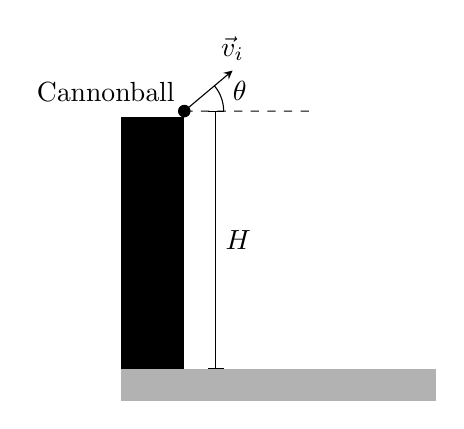
\begin{tikzpicture}[>=stealth,scale=0.8]
  \fill[black] (0,0) rectangle (-1,4);
  \coordinate (C) at (0,4.1);
  \fill (C) circle (0.1) node [above left]{Cannonball};
  \coordinate (vi) at ($(C)+(40:1)$);
  \coordinate (h) at ($(C)+(0:2)$);
  \draw[->] (C) -- (vi) node [above]{$\vec{v}_i$};
  \draw[dashed] (C) -- (h);
  \fill[black!30!white] (-1,-0.5) rectangle (4,0);
  \draw pic ["$\theta$",draw,angle eccentricity=1.5] {angle = h--C--vi};
  \draw [|-|] (0.5,0) -- +(0,4.1) node [midway, right]{$H$};
\end{tikzpicture}

\begin{enumerate}[resume]
  \item Based on your coordinate system, write a vector for the initial position and the
  initial velocity in terms of the given quantities $H,\theta$ and the magnitude of the initial
  velocity $\left|\vec{v}_i\right| = v_i$:
  \[
    \vec{r}_i = (x_i, y_i) = \hspace{1.5in} \vec{v}_i = \left(v_{ix},v_{iy}\right) = \hspace{1in}
  \]
  \item Draw a free body diagram for a projectile shortly after it has been fired by the
  cannon. (For today, ignore air resistance). \vspace{0.5in}
  \item Write an algebraic expression for each of the components of your
  acceleration. \vspace{0.5in}
  \item Based on this information, write general equations allowing you to calculate each
  component of the position and velocity vectors at any time $t$:
  \begin{align*}
    x(t) &= \phantom{X} \hspace{5in} \phantom{X} \\
    y(t) &= \\
    v_x(t) &= \\
    v_y(t) &= \\
  \end{align*}
\end{enumerate}

\vfill
{\Large \ding{237} Check your answers with an instructor before continuing!}

\newpage
\section{Measuring the height of the cliff}
\begin{enumerate}
  \item If we assume a cliff height $H$, launch speed $v_i$ and launch angle $\theta$, write an
  algebraic expression determining the time $T$ that a projectile will hit the
  ocean. \vspace{0.5in}
\end{enumerate}
\begin{tcolorbox}[colback=black!5!white,colframe=white!15!black,title=More information]
  In order to determine the height of the cliff, you grab a rock, a stopwatch, and your trusty
  binoculars and go to the edge of the cliff. You then drop the rock and start your watch
  simultaneously. Carefully following the fall of the rock in your binoculars, you stop your
  watch at the instant that you see the splash and find that the rock hit the water
  \SI{5.0}{\second} later. 
\end{tcolorbox}

\begin{enumerate}[resume]
  \item Using the above information, determine the height of the cliff and the speed of the
  rock when it hit the ocean. \vspace{0.5in}
\end{enumerate}

\section{Calculate the Range}
\begin{tcolorbox}[colback=black!5!white,colframe=white!15!black,title=More information]
  You have been looking through the archives and find a reference to the muzzle velocity of the
  cannon, finding a value of \SI{60.0}{\meter\per\second}. You aren't sure how accurate that
  is, so you want to leave this value as a parameter you can change in the calculations below.
\end{tcolorbox}

\begin{enumerate}
  \item Write a code with the following given/constant variables:
  \begin{itemize}
    \item Gravitational acceleration $g$
    \item Muzzle velocity $v_i$
    \item Launch angle $\theta$
  \end{itemize}
  and the following calculated variables:
  \begin{itemize}
    \item Time-in-flight $T$
    \item Cliff height $H$
  \end{itemize}
  That allows you to calculate the position vector $(x,y)$, velocity vector $(v_x,v_y)$,
  acceleration vector $(a_x, a_y)$, and speed $v=\sqrt{v_x^2 + v_y^2}$ at 100 instants that
  occur while the object is in flight.
  \item From your code, create the following plots:
  \begin{itemize}
    \item $x$ vs.\ $t$ and $y$ vs.\ $t$
    \item $v_x$ vs.\ $t$ and $v_y$ vs.\ $t$
    \item $a_x$ vs.\ $t$ and $a_y$ vs.\ $t$
  \end{itemize}
  \item Using your code, and the given numerical values, determine to the nearest degree the
  launch angle that will give the maximum range of the cannon.
\end{enumerate}

On Friday, you need this code, we'll start with it as a baseline when we talk about adding in
air resistance. And we'll bring back our friend the Euler method.
\end{document}

